En el diagrama de contexto se ve quiénes se relacionan con UteqFit-AI y qué se pasa con cada uno.

Los estudiantes mandan su reserva y su pedido de rutina, y reciben los horarios disponibles y la rutina revisada. El encargado del gimnasio registra las entradas y salidas, y recibe las reservas y el aforo. El responsable en UBU recibe el seguimiento del servicio. La Dirección de Bienestar da la autorización y recibe la supervisión del servicio. TICs entrega la hoja de inscripción.

\begin{figure}[H]
  \centering
  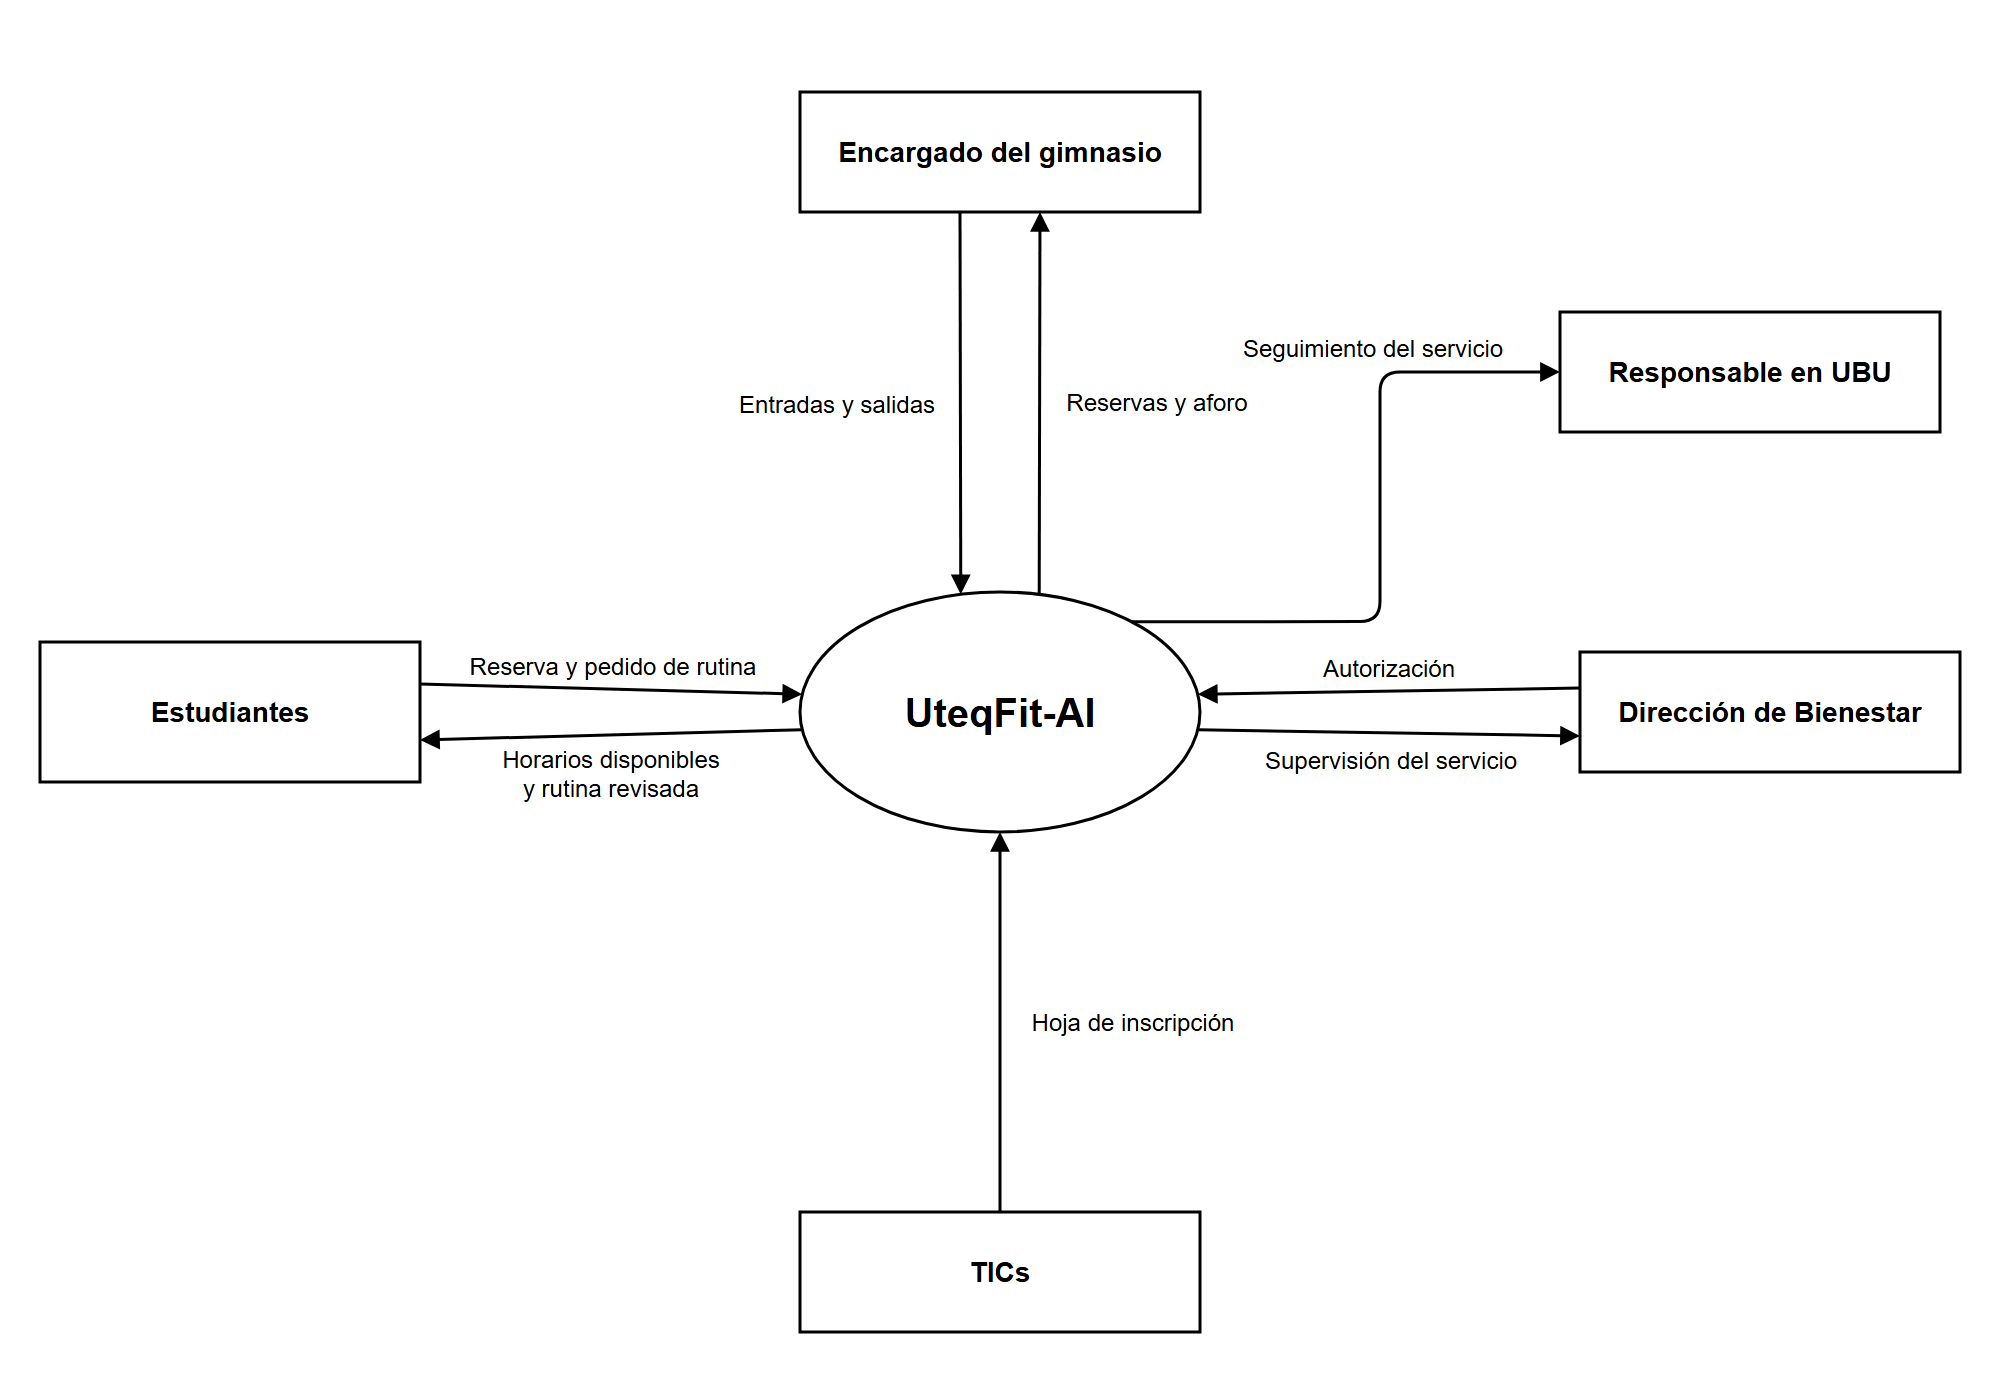
\includegraphics[width=0.95\textwidth]{figuras/diagrama_contexto.png}
  \caption{Diagrama de contexto de UteqFit-AI}
  \label{fig:diagrama-contexto}
\end{figure}

\subsection{Perspectivas del contexto}

En la Tabla~\ref{tab:perspectivas} se pone un hallazgo por cada una de las ocho perspectivas de contexto de Pohl~\cite{pohl2025}, sacado de lo que ya se observó en el gimnasio.

\begingroup
\small
\renewcommand{\arraystretch}{1.2}
\begin{longtable}{|p{2.6cm}|p{8.6cm}|p{3.2cm}|}
\caption{Hallazgos por perspectiva}\label{tab:perspectivas}\\\hline
\textbf{Perspectiva} & \textbf{Hallazgo} & \textbf{De dónde sale} \\ \hline
\endfirsthead
\hline \textbf{Perspectiva} & \textbf{Hallazgo} & \textbf{De dónde sale} \\ \hline
\endhead
Uso & Para entrar se presenta la cédula o el carné y se registra a mano en la entrada. Algunos estudiantes se quedan después de su hora. & Afiche y observación O3 \\ \hline
Sujeto o dominio & El cupo máximo es de 26 personas por hora, y el gimnasio atiende de 08h00 a 13h00 y de 15h00 a 18h00. & Observación O2 y afiche \\ \hline
Sistema de TI & Hoy no hay ningún sistema: TICs entrega la hoja de inscripción y todo se hace a mano. & Observación O1 \\ \hline
Desarrollo & Es un proyecto académico que llega hasta los requisitos y una prueba piloto antes de la semana 17. & Secciones 2 y 7 \\ \hline
Negocio & El gimnasio es gratuito y depende de Bienestar Universitario, así que el sistema no maneja cobros. & Sección 1 \\ \hline
Innovación & Hubo entre 4 y 5 pedidos de ayuda con rutinas y no hay entrenador. Una rutina sugerida tendría que aprobarla el responsable que designe UBU. & Observación O5 y riesgo R-04 \\ \hline
Sociedad & El sistema guarda datos personales de los estudiantes, por eso se aplica la LOPDP y no se guardan datos de salud. & Secciones 2 y 6 \\ \hline
Técnica & Todavía no se sabe con qué equipos y red cuenta el gimnasio, y la conexión con los servicios de TICs está por definir. & Sección 2 (zona gris) \\ \hline
\end{longtable}
\endgroup
